\documentclass[12pt,a4paper,twoside,openright,titlepage,final]{article}
\usepackage{fontspec}
\usepackage{amsmath}
\usepackage{amsfonts}
\usepackage{amssymb}
\usepackage{makeidx}
\usepackage{graphicx}
\usepackage[hidelinks,unicode=true]{hyperref}
\usepackage[spanish,es-nodecimaldot,es-lcroman,es-tabla,es-noshorthands]{babel}
\usepackage[left=3cm,right=2cm, bottom=4cm]{geometry}
\usepackage{natbib}
\usepackage{microtype}
\usepackage{ifdraft}
\usepackage{verbatim}
\usepackage[obeyDraft]{todonotes}
\ifdraft{
	\usepackage{draftwatermark}
	\SetWatermarkText{BORRADOR}
	\SetWatermarkScale{0.7}
	\SetWatermarkColor{red}
}{}
\usepackage{booktabs}
\usepackage{longtable}
\usepackage{calc}
\usepackage{array}
\usepackage{caption}
\usepackage{subfigure}
\usepackage{footnote}
\usepackage{url}
\usepackage{tikz}
\tikzset{
  treenode/.style = {shape=rectangle, rounded corners,
                     draw, align=center,
                     top color=white, bottom color=blue!20},
  root/.style     = {treenode, font=\Large, bottom color=red!30},
  env/.style      = {treenode, font=\ttfamily\normalsize},
  dummy/.style    = {circle,draw}
}

\setsansfont[Ligatures=TeX]{texgyreadventor}
\setmainfont[Ligatures=TeX]{texgyrepagella}

%*******************************************************
%                 NO MODIFICAR
\newcommand*{\FSfont}[1]{%
  \fontencoding{T1}\fontfamily{#1}\selectfont}

\newlength{\tpheight}\setlength{\tpheight}{0.9\textheight}
\newlength{\txtheight}\setlength{\txtheight}{0.9\tpheight}
\newlength{\tpwidth}\setlength{\tpwidth}{0.9\textwidth}
\newlength{\txtwidth}\setlength{\txtwidth}{0.9\tpwidth}
\newlength{\drop}
%*******************************************************

% Crea una portada con los siguientes parámetros
%
% #1 : Título 
% #2 : Subtítulo
% #3 : Subsubtítulo
% #4 : Autor(es)
% #5 : Lugar
%

\newcommand*{\portada}[5]{
\begin{titlepage}
\begingroup
\vspace*{1cm}
\drop = 0.2\txtheight
\centering
\vfill
{\Huge \scshape #1}\\[\baselineskip]
{\Large \textbf{#2}}\\[\baselineskip]
{\Large \scshape #3}\\[\baselineskip]
\vspace*{0.3cm}
{\large \textit{#4}}\\[0.5\drop]

\includegraphics[scale=0.35]{./imagenes/logoURJC.jpg}
\vspace*{1.5cm}

{\large \scshape #5, \today} \par
\begin{center}
\end{center}
\vfill\null
\endgroup
\end{titlepage}
}
 %*****************************************************
 


\author{José Ignacio Escribano}

\title{Caso práctico II}

\setlength{\parindent}{0pt}

\begin{document}

\pagenumbering{alph}
\setcounter{page}{1}

\portada{Caso Práctico II}{Modelización y tratamiento de la incertidumbre}{Probabilidades y variables aleatorias}{José Ignacio Escribano}{Móstoles}

\listoffigures
\thispagestyle{empty}
\newpage

\tableofcontents
\thispagestyle{empty}
\newpage


\pagenumbering{arabic}
\setcounter{page}{1}

\section{Introducción}

La empresa WEBSYMASWEBS quiere conocer la calidad de las conexiones, midiendo el número de intentos hasta concertarse a una página web. Para ello contrata a una consultora para que hagan el informe. Además de la conexión, se mide el tráfico que se genera al realizar la conexión, y el grado de satisfacción de los clientes a través de una serie de cuestionarios.

\section{Resolución del caso práctico}

A continuación resolveremos las tres partes de las que consta el caso práctico: la primera es sobre el número de intentos al acceder a la página web; la segunda es de el tráfico que se registró al acceder a la página web; y la tercera, sobre una encuesta que se hizo para conocer el grado de satisfacción 

\subsection{Tarea I}

La calidad de la conexión a una página web se mide mediante el número de intentos (incluido el exitoso) hasta que se consigue acceder a la página web. Existen tres niveles de calidad: conexión EXCELENTE, BUENA y MALA.\\
Se tiene una conexión EXCELENTE si se han necesitado 2 ó menos intentos, BUENA si se han necesitado 3 ó 4 intentos y, MALA si se han necesitado más de 5 intentos para conectarse a la página web.\\

De los 50 datos recogidos por la empresa, 35 corresponden a la conexión EXCELENTE, 13 a la conexión BUENA, y 2 corresponden a la conexión MALA. En porcentaje, el 70\% corresponden con la conexión EXCELENTE, el 26\% con la conexión BUENA y, el 4\% con la conexión MALA.\\

Para calcular la probabilidad de que un cliente necesite más de 7 intentos necesitamos la frecuencia absoluta de cada uno de los valores del soporte:

\begin{table}[htbp]
\centering
\begin{tabular}{|c|c|}
\hline Número de intentos & Frecuencia absoluta \\ 
\hline 1 & 25 \\ 
\hline 2 & 10 \\ 
\hline 3 & 9 \\ 
\hline 4 & 4 \\ 
\hline 5 & 2 \\ 
\hline 
\end{tabular} 
\end{table}

Así pues, la probabilidad viene dada por

\[ P(X \geq 7) = 1 - P(X < 6) = 1 - \sum_{k=1}^{5} P(X = k) = 1 - \left(  \dfrac{25}{50} + \dfrac{10}{50} + \dfrac{9}{50} + \dfrac{4}{50} + \dfrac{2}{50} \right) = 0  \]

\subsection{Tarea II}

A parte de los datos del número de intentos para acceder a la página web, también se han recogido datos sobre el tráfico de datos que se generó durante la conexión, medidos en kilobytes. También se han creado tres categorías para clasificar a sus clientes: A = ``Tráfico BAJO'', B = ``Tráfico MEDIO'' y C = ``Tráfico ALTO'', pero estos datos se han perdido a un fallo al realizar la copia de seguridad, aunque se recuerdan que los datos seguía una distribución normal de media 250 y desviación típica 60.\\

La empresa desea que en cada categoría se halle exactamente un tercio de sus clientes. Para obtener los bordes de las distintas regiones, calculamos los percentiles que acumulan a su izquierda un 1/3 y 2/3 de probabilidad. Estos datos se corresponden con los valores 224.1564 y 275.8436, respectivamente. En la Figura~\ref{fig:distribucion_normal} se muestra la distribución normal, junto con cada una de las regiones.\\

\begin{figure}[htbp!]
\centering
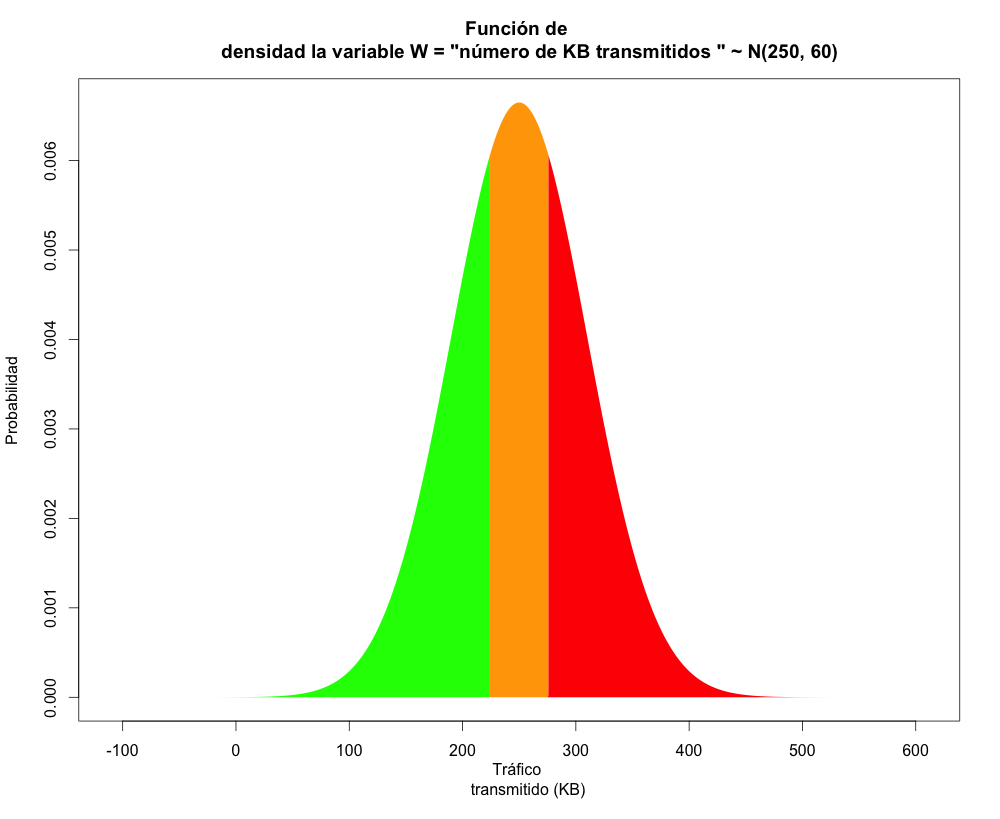
\includegraphics[width=0.8\linewidth]{./imagenes/distribucion_normal}
\caption{Distribución normal con media 250 y desviación típica 60. Se muestran tres zonas: la verde correspondiente con la categoría Tráfico BAJO; la naranja, con la categoría Tráfico MEDIO; y, la roja, con la categoría Tráfico ALTO. Cada una de las regiones tiene un tercio de probabilidad.}
\label{fig:distribucion_normal}
\end{figure}

Por tanto, si denotamos con $W$ el número de kilobytes trasmitidos, las categorías vienen dadas por el siguiente criterio:

\[\text{Tráfico} \begin{cases}
\text{BAJO} & \text{si } W \leq 224.1564 \\
\text{MEDIO} & \text{si } 224.1564 < W \leq 275.8436 \\
\text{ALTO} & \text{si } W > 275.8436
 
\end{cases}\]

Además de las regiones, se necesitan calcular una serie de probabilidades:

\begin{itemize}
\item Probabilidad de que un cliente tenga una conexión MALA y haya generado un tráfico BAJO.

\begin{align*}
P(\text{MALA} \cap \text{BAJO}) &=  P(\text{MALA}) \cdot P(\text{BAJO})\\ &= P(\text{MALA}) \cdot P(W \leq 224.1564)\\ &= 0.04 \cdot 0.333 \\ &= 0.0133
\end{align*}

La probabilidad $P(\text{MALA})$ viene dada por el porcentaje calculado en la Tarea I, y la probabilidad $P(\text{BAJO})$ se ha calculado con R. Se ha supuesto independencia porque así lo supone el enunciado.

\item Probabilidad de que, de 10 clientes seleccionados al azar, al menos 9 de ellos tengan conexión BUENA o EXCELENTE.

Primero, calculamos la probabilidad de un cliente, elegido al azar, tenga conexión BUENA o EXCELENTE.

\begin{multline*}
P(\text{BUENA} \cup \text{EXCELENTE}) = P(\text{BUENA}) + P(\text{EXCELENTE}) \\ - P(\text{BUENA} \cap \text{EXCELENTE})
\end{multline*}

Pero, como tener una conexión BUENA y tener una conexión EXCELENTE son sucesos disjuntos tenemos que $P(\text{BUENA} \cap \text{EXCELENTE}) = 0$.\\

Por tanto, 

\begin{align*}
P(\text{BUENA} \cup \text{EXCELENTE}) &= P(\text{BUENA}) + P(\text{EXCELENTE}) \\ &= 0.70 + 0.26 \\ &= 0.96
\end{align*}

Ambas probabilidades vienen dadas por los porcentajes calculados en la Tarea I.\\

Nos queda calcular la probabilidad de que al menos 9 de 10 clientes, tengan una conexión BUENA o EXCELENTE.\\

En este caso, tenemos una distribución binomial con $n = 10$ y $p = 0.96$, que acabamos de calcular.\\

Por tanto, si llamamos $H$ al número de clientes tenga una conexión BUENA o EXCELENTE,

\begin{align*}
P(H \geq 9) &= 1 - P(H < 9) \\ &=  1 - P(H \leq 8) \\ &= 1 - 0.058 \\ &= 0.941  
\end{align*}

\item Probabilidad de que, de 10 clientes seleccionados al azar, no haya ninguno que tenga conexión EXCELENTE y haya generado un tráfico BAJO.

Primero, calculamos la probabilidad de un cliente tenga conexión EXCELENTE y haya generado un tráfico BAJO.

\begin{align*}
P(\text{EXCELENTE} \cap \text{BAJO}) &= P(\text{EXCELENTE}) \cdot P(\text{BAJO}) \\ &= 0.7 \cdot P(W \leq 224.1564) \\ &= 0.7 \cdot 0.333 \\ & = 0.233 
\end{align*} 

De nuevo, volvemos a suponer independencia entre ambas variables.\\

Nos queda calcular la probabilidad de que, entre 10 clientes elegidos al azar, no haya ninguno que tenga una conexión EXCELENTE y haya generado un tráfico BAJO.\\

Como en el caso anterior tenemos una distribución binomial con $n = 10$ y $p = 0.233$.\\

Sea $H$ el número de clientes que tenga una conexión EXCELENTE y haya generado un tráfico BAJO. Entonces, la probabilidad pedida es

\begin{align*}
P(H = 0) = 0.070
\end{align*}   
\end{itemize}

\subsection{Tarea III}

Por último, se desea saber el grado de satisfacción de los clientes. Para ello, se distribuyen cuatro cuestionarios ($C_1$, $C_2$, $C_3$ y $C_4$). El cuestionario $C_1$ se ha distribuido al 40\% de los clientes, el $C_2$ al 30\%, el $C_3$ al 20\% y, el $C_4$ al 10\%. El porcentaje de clientes que no ha respondido al cuestionario es del 1\%, 2\%, 7\% y 4\%, respectivamente.\\

De nuevo, se piden una serie de probabilidades relativas a los cuestionarios.\\

Antes de calcular las probabilidades hacemos el modelo gráfico, que se muestra en la Figura~\ref{fig:modelo_grafico}.

\begin{figure}[htbp!]
\centering
\begin{tikzpicture}
  [
    grow                    = right,
    level distance=20mm,
	text depth=.1em,
	text height=.8em,
	level 1/.style={sibling distance=5em},
	level 2/.style={sibling distance=2em},
    edge from parent/.style = {draw, -latex},
    every node/.style       = {font=\footnotesize},
    sloped
  ]
  \node {}
     child { node [env] {$C_1$}
           child { node [env] {$C$}
             edge from parent node [below] {$0.99$} } 
           child { node [env] {$NC$}
             edge from parent node [above] {$0.01$} }
           edge from parent node [above] {$0.4$} }
     child { node [env] {$C_2$}
           child { node [env] {$C$}
             edge from parent node [below] {$0.98$} } 
           child { node [env] {$NC$}
             edge from parent node [above] {$0.02$} }
           edge from parent node [above] {$0.3$} }   
     child { node [env] {$C_3$}
           child { node [env] {$C$}
             edge from parent node [below] {$0.93$} } 
           child { node [env] {$NC$}
             edge from parent node [above] {$0.07$} }
           edge from parent node [above] {$0.2$} } 
     child { node [env] {$C_4$}
           child { node [env] {$C$}
             edge from parent node [below] {$0.96$} } 
            child { node [env] {$NC$}
              edge from parent node [above] {$0.04$} }
           edge from parent node [above] {$0.1$} };
\end{tikzpicture}
\caption{Modelo gráfico de la Tarea III. $C_i$ denota el suceso de recibir el cuestionario $C_i$ con $i = 1,2,3,4$, $NC$ es el suceso de no contestar al cuestionario, y $C$ es el suceso de contestar al cuestionario}
\label{fig:modelo_grafico}
\end{figure}

\begin{itemize}
\item Si elegimos un cliente al azar, ¿cuál es la probabilidad de que haya contestado al cuestionario?

Si denotamos con $C$ al suceso de contestar el cuestionario, la probabilidad la calculamos aplicando el Teorema de la Probabilidad Total. Así la probabilidad es

\begin{align*}
P(C) &= 0.4 \cdot 0.99 + 0.3 \cdot 0.98 + 0.2 \cdot 0.93 + 0.1 \cdot 0.1 \cdot 0.96 \\ &= 0.972
\end{align*} 

\item Si elegimos un cliente al azar y resulta que no ha contestado a su cuestionario, ¿qué cuestionario es más probable que hubiese recibido, $C_1$, $C_2$, $C_3$ o $C_4$?

Si denotamos con $NC$ al hecho de no contestar el cuestionario y con $C_i$ al suceso de recibir el cuestionario $C_i$. Entonces, aplicamos el teorema de Bayes para cada uno de los cuestionarios.

\begin{align*}
P(C_1 | NC) & = \dfrac{P(NC | C_1) \cdot P(C_1)}{P(NC)} = \dfrac{0.01 \cdot 0.4}{0.028} = 0.142 \\
P(C_2 | NC) & = \dfrac{P(NC | C_2) \cdot P(C_2)}{P(NC)} = \dfrac{0.02 \cdot 0.3}{0.028} = 0.214 \\
P(C_3 | NC) & = \dfrac{P(NC | C_3) \cdot P(C_3)}{P(NC)} = \dfrac{0.07 \cdot 0.2}{0.028} = 0.500 \\
P(C_4 | NC) & = \dfrac{P(NC | C_4) \cdot P(C_4)}{P(NC)} = \dfrac{0.04 \cdot 0.1}{0.028} = 0.142
\end{align*}

La probabilidad $P(NC)$ se puede calcular aplicando el Teorema de la Probabilidad Total, o bien, como suceso complementario al suceso de contestar el cuestionario.\\

Por tanto, lo más probable es que contestara al cuestionario $C_3$.

\item Si tomamos 4 clientes al azar, ¿cuál es la probabilidad de que al menos haya un cuestionario sin contestar?

La probabilidad $P(NC) = 0.028$, ya está calculada anteriormente. Por lo que debemos considerar una distribución binomial con $n = 4$ y $p = 0.028$.\\

\begin{align*}
P(NC \geq 1) &= 1 - P(NC < 1) \\ &= 1 - P(NC = 0) \\ &= 1 - 0.892 \\ &= 0.107
\end{align*}  

\item Misma pregunta que el caso anterior si la muestra es de 200 clientes.

Repetimos lo mismo que en caso anterior, pero teniendo en cuenta que ahora nuestra distribución binomial tiene como parámetros $n = 200$ y $p = 0.028$.

\begin{align*}
P(NC \geq 1) &= 1 - P(NC < 1) \\ &= 1 - P(NC = 0) \\ &= 1 - 0.003 \\ &= 0.997
\end{align*}

\end{itemize}

\section{Conclusiones}

En este caso práctico hemos puesto en práctica la teoría del cálculo de probabilidades así como los teoremas clásicos de ésta (Teorema de la Probabilidad Total y el Teorema de Bayes). También hemos utilizado dos de las distribuciones más usadas: la distribución normal y la distribución binomial. Para calcular las probabilidades pedidas, nos valimos de R para calcular éstas de forma fácil y eficiente.    

\newpage

\section{Código R}

\verbatiminput{../caso_ii.R}


\end{document} 